\documentclass[12pt]{report}
\usepackage{graphicx}
\usepackage{hyperref}

\title {
	
\includegraphics[width = .2\linewidth]{University-of-Lugano.png} \break \break
	{\bf\Huge Contextual Inquiry and Analysis}
	\\\large Human-Computer Interaction
	\\\small Academic Year 2017/2018 \break
	\\\large \textbf{Group 7}}
	\author{
	\\\large Alessandra Vicini \\ Edoardo Lunardi \\ Ozren Dabic \\ Pasquale Polverino \\ Paganoni Marco}
\date{March 12, 2018}
\begin{document}
	\pagestyle{empty}
	\maketitle
	\section*{\huge Our Research}
	We envisioned an application with which children could organize meetings
	with each other based on their interests, such as the sports they play, 
	or what they do in their free time. We were aware of the fact 
	that our users are minors and, keeping this in mind, we tried to develop 
	our idea around this, keeping in mind all the challenges and drawbacks 
	that come with developing an app for children. The "field visit" allowed us to properly
	understand what children expect from our application. During the interview we asked
	them about some of the features that we should include in the app. 
	We initially asked for information regarding their interests, so that
	we would gather enough data to aid the development of our product. 
	We also faced the problem of the usage of smartphone: many children have some limitations, either
	imposed by parents and/or by the school, which does not allow children
	to use their phone during certain time periods. Finally we revealed our idea to
	ensure that the application can be used only by children: we
	proposed that the access accounts may be given only by the school, and the
	children supported this. So in short, our "field visit" has
	asserted our ideas for the app and the children gave us some suggestions,
	which means a lot to us as far as future development is concerned.\\

	Upon reading the interviews from the remaining groups, we noticed 
	a similarity in the questions asked. However, some were too vague, 
	and the information gathered from these questions was discarded, 
	since it is not relevant to what we envisioned to develop. 
	Because of this, we tried to construct our flow model with the goal 
	representing all our users, showcasing information on them, 
	as well as their expectations, in order to satisfy their demands.\\

	By analysing all the interviews, we organized our work activity affinity diagram 
	grouping the main points we have found into 9 bigger subsets. 
	Then we classified all the data gathered from the interviews into each of the subsets. 
	
	Our subsets were mainly based on the responses provided by the children, 
	as well as topics argued in class, for instance the privacy and safety of 
	applications that use private information.
	
	In the end our diagram revolves around three main concepts: 
	what our clients expect from the app, how we can deal with this, by creating something which attracts them 
	and lastly ethical problems, which must be taken in consideration since we are talking about
	children. Our work looked this way: \\\\\\
	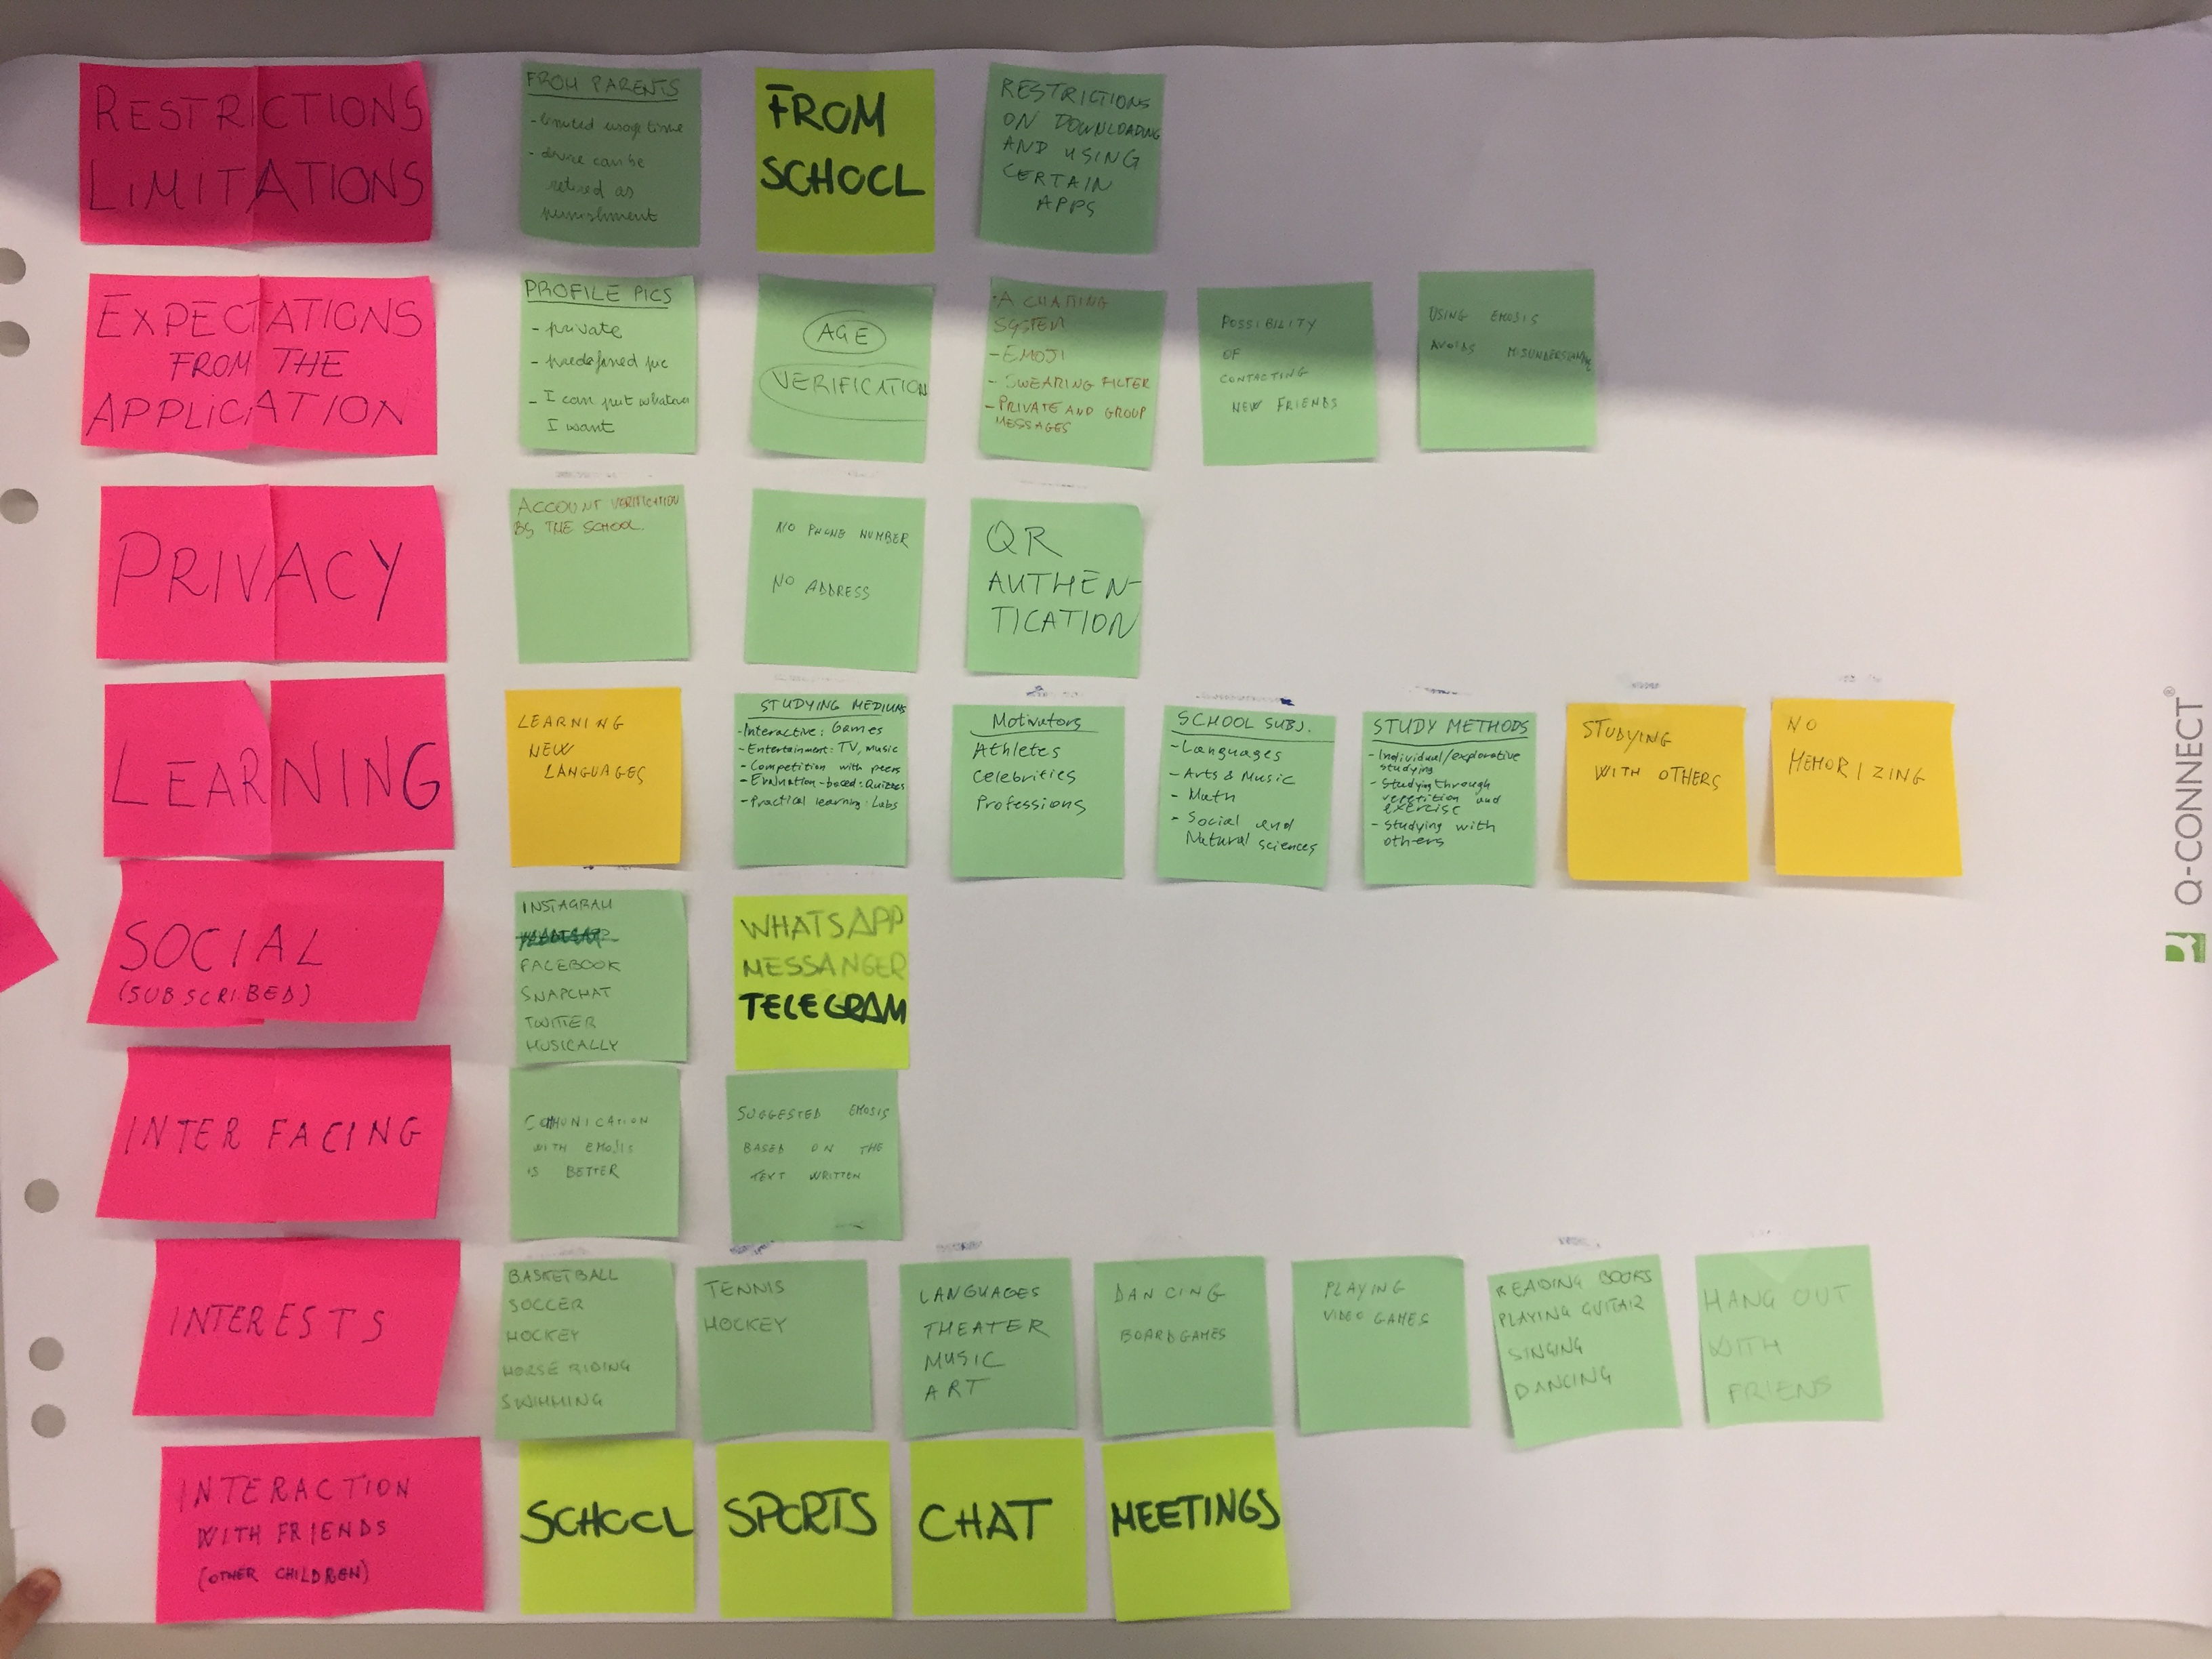
\includegraphics[width = 1.0\linewidth]{affinity_diagram.jpg}\break

  As clearly visible in the diagram we create 9 subsets and each of them has its
  main topics. These subsets include:
	\begin{itemize}
		\item "Restrictions and Limitations":\\
		       we created this subset because we noticed that most children have
					 restrictions and limitations regarding the usage of their phones.
		\item "Expectations from the application" :\\
		       this was an obvious topic to take into consideration. It is our duty to listen to the requests and expectations of our users. 
					 We also noticed that some of their expectations matched our initial product idea.
		\item "Privacy":\\
		       that is the main ethical problem, and just because our users will be children,
					 we place a higher emphasis on this part, and present alternatives which will allow the app to be more safer and reliable.
		\item "Learning":\\
		       some children expect an application which will help them to learn new things, so even if this wasn't
					 part of our original idea we could think of implementing something akin to that.
		\item "Social":\\
		       this point revolves around famous design characteristics that other social apps use. If children are more familiar
					 with a certain type of design, we will try to create something both similar as well as improve on the popular design.
		\item "Interfacing":\\
		       many children suggested the usage of emojis in communication. Our app will include a sort
					 of live chat, so this is a great suggestion for us.
		\item "Interests":\\
		       this is the meat of our application, so we listed the most common interests and hobbies
					 so that we can include them in our product. Knowing what our users do allows us to better categorise them, as well as to pair them up accordingly.
		\item "Interaction with friends:"\\
		       we make sure that children are used to go out with friends and they have the possibility to do
					 so and if not, why not and try to solve the problem?

	\end{itemize}

	 This was our analysis of the project in the entire context, keeping in mind who our users are and what we
	 plan to do in order to meet their demands. Each part of the project has been structured having the children in mind. All the information that we have has been gathered through the interview. Our group worked together to reach the best result possible, and we are all satisfied.

	\end {document}